%%%%%%%%%%%%%%%%%%%%%%%%%%%%%%%%%%%%%%%%%%%%%%%%%%%%%
%% Use a minimum font size of 12pt and specify a4paper
%% for ease of display and printing in the UK
%%%%%%%%%%%%%%%%%%%%%%%%%%%%%%%%%%%%%%%%%%%%%%%%%%%%%
\documentclass[12pt,a4paper]{article}

%%%%%%%%%%%%%%%%%%%%%%%%%%%%%%%%%%%%%%%%%%%%%%%%%%%%%
%% Geometry package to change margins etc.
%%%%%%%%%%%%%%%%%%%%%%%%%%%%%%%%%%%%%%%%%%%%%%%%%%%%% 
\usepackage[a4paper,margin=2.5cm]{geometry}

%%%%%%%%%%%%%%%%%%%%%%%%%%%%%%%%%%%%%%%%%%%%%%%%%%%%%
%% Babel package to specify English typographical 
%% rules, and hyphenation patterns
%%%%%%%%%%%%%%%%%%%%%%%%%%%%%%%%%%%%%%%%%%%%%%%%%%%%%
\usepackage[english]{babel}

%%%%%%%%%%%%%%%%%%%%%%%%%%%%%%%%%%%%%%%%%%%%%%%%%%%%%
%% T1 font encoding to ensure characters with accents 
%% and other non-ascii characters can be correctly 
%% searched, copied and pasted in the PDF output. Also 
%% enables hyphenation of words containing letters 
%% with accents.
%%
%% Note, you should have cm-super installed otherwise
%% computer modern fonts will be bitmaps. 
%% If this is a problem then move this command inside
%% a clearprint toggle below. 
%%%%%%%%%%%%%%%%%%%%%%%%%%%%%%%%%%%%%%%%%%%%%%%%%%%%%
\usepackage[T1]{fontenc}

%%%%%%%%%%%%%%%%%%%%%%%%%%%%%%%%%%%%%%%%%%%%%%%%%%%%%
%% This is the master for 3 document formats.
%% We DO NOT support compiling via latex-dvips-ps2pdf. 
%% If you wish to use diagrams which rely on this 
%% then these should be produced as standalone figures 
%% in PDF and svg formats and included in the LaTeX
%% via the graphicx package.
%%
%% Standard print: Compiled via pdflatex. You can 
%% style how you provided you can compile the other
%% formats.
%% 
%% Clearprint: Compiled via pdflatex. 
%%
%% Accessible web pages via TeX4ht with MathJax
%% as the renderer: for zoom, magnification, text to 
%% speech (TextHelp Read & Write), screenreaders 
%% (NVDA, JAWS 16+, ChromeVox, other Aria aware), 
%% electronic braille (NVDA), also good on small 
%% screens. 
\usepackage{etoolbox}
\newtoggle{clearprint}
\newtoggle{web}
%% The below uses the make file to determine which 
%% format to compile. Please note that compilation 
%% requires a post-2009 version of etoolbox and, for 
%% the web format, a working copy of TeX4ht. 
%% Using the makefile is the recommended compilation 
%% method as this will produce a single zip containing
%% the web format for you. 
\togglefalse{clearprint}\toggletrue{web}

%% If you are NOT using the make file you may 
%% uncomment one of the below:
%%
%% Standard print PDF. Compiled via pdflatex:
%\togglefalse{clearprint}\togglefalse{web}
%%
%% Clear print PDF. Compiled via pdflatex: 
%\toggletrue{clearprint}\togglefalse{web}
%%
%%Accessible web format. Requires TeX4ht - see 
%% make file for commands to run: 
%\togglefalse{clearprint}\toggletrue{web}
%%%%%%%%%%%%%%%%%%%%%%%%%%%%%%%%%%%%%%%%%%%%%%%%%%%%%

%%%%%%%%%%%%%%%%%%%%%%%%%%%%%%%%%%%%%%%%%%%%%%%%%%%%%
%% Standard packages loaded.
%%%%%%%%%%%%%%%%%%%%%%%%%%%%%%%%%%%%%%%%%%%%%%%%%%%%%
%% Only graphicx and the picture environment can 
%% be used for graphics.  
\usepackage{amsmath,amssymb,amsfonts,amsthm}
\usepackage{hyperref}
%%
%% Graphicx must be loaded whether used or not as 
%% TeX4ht compilation expects it.
%% We can deal with EPS figures but this is not 
%% covered in this example.  
\usepackage{graphicx}
\graphicspath{{./figures/}} 
%%%%%%%%%%%%%%%%%%%%%%%%%%%%%%%%%%%%%%%%%%%%%%%%%%%%%
%% Other packages may not work for this process.
%% See the second example for further packages. 
%%%%%%%%%%%%%%%%%%%%%%%%%%%%%%%%%%%%%%%%%%%%%%%%%%%%%

%%%%%%%%%%%%%%%%%%%%%%%%%%%%%%%%%%%%%%%%%%%%%%%%%%%%%
%% Requirements for clearprint/web version
%%%%%%%%%%%%%%%%%%%%%%%%%%%%%%%%%%%%%%%%%%%%%%%%%%%%%
\ifboolexpr{togl {clearprint} or togl {web}}{
%% Change font to Helvetica and heavier verbatim font
\renewcommand{\familydefault}{phv}
\fontfamily{phv}\selectfont
\usepackage[scaled=0.95]{DejaVuSansMono}

%% Emphasis in bold only - add additional examples 
%% as per resource
\renewcommand{\em}{\bf}
\renewcommand{\textit}{\textbf}
\renewcommand{\emph}{\textbf}
\renewcommand{\it}{\bf }

%% Additional spacing - may not be honoured in 
%% web version
\setlength{\parindent}{0.0pt}
\setlength{\parskip}{1.0\baselineskip}
\renewcommand{\baselinestretch}{1.25}\selectfont
\mathsurround 0.2em
\setlength{\arraycolsep}{0.5cm}\renewcommand{\arraystretch}{1.25}
\addtolength{\jot}{0.5\baselineskip}
\sloppy
\allowdisplaybreaks
}
%%%%%%%%%%%%%%%%%%%%%%%%%%%%%%%%%%%%%%%%%%%%%%%%%%%%%

%%%%%%%%%%%%%%%%%%%%%%%%%%%%%%%%%%%%%%%%%%%%%%%%%%%%%
%% Commands used to provide alternative text for 
%% diagrams for a screenreader user.
%% DO NOT remove the macros from the preamble even if
%% you are not using them as the web compilation 
%% expects them to be defined.
\newcommand{\nextalt}[1]{} 
\newcommand{\PICalt}[1]{{#1}} 
%%%%%%%%%%%%%%%%%%%%%%%%%%%%%%%%%%%%%%%%%%%%%%%%%%%%%

%%%%%%%%%%%%%%%%%%%%%%%%%%%%%%%%%%%%%%%%%%%%%%%%%%%%%
%% You can style your theorems etc. as you like but 
%% in clearprint and accessible web use a clearprint 
%% style to open up spacing, use bold for emphasis 
%% and to avoid large parts of text in italics. 
\ifboolexpr{togl {clearprint} or togl {web}}
{
\newtheoremstyle{clearprint}
{20pt}% space above
{3pt}% space below
{}% body font
{}% indent amount
{\bfseries}% theorem head font
{.\newline }% punctuation after theorem head
{1.0em}% space after theorem head
{}% theorem head spec, can be left empty meaning normal
\theoremstyle{clearprint}
\newenvironment{Proof}
{\noindent{\bf Proof.}\hspace*{1em}}% Begin
{\qed\par}% End
}
%%%%%%%%%%%%%%%%%%%%%%%%%%%%%%%%%%%%%%%%%%%%%%%%%%%%%
%% Leave a blank line after this

%%%%%%%%%%%%%%%%%%%%%%%%%%%%%%%%%%%%%%%%%%%%%%%%%%%%%
%% In default style in standard print
\newtheorem*{example*}{Example}
%%%%%%%%%%%%%%%%%%%%%%%%%%%%%%%%%%%%%%%%%%%%%%%%%%%%%

%%%%%%%%%%%%%%%%%%%%%%%%%%%%%%%%%%%%%%%%%%%%%%%%%%%%%
%% Change to definition style for the standard print
\ifboolexpr{togl {clearprint} or togl {web}}
{\theoremstyle{clearprint}}
{\theoremstyle{definition}}
%% Leave a blank line after this

%%%%%%%%%%%%%%%%%%%%%%%%%%%%%%%%%%%%%%%%%%%%%%%%%%%%%
%% In definition style unless in clearprint
\newtheorem*{definition*}{Definition}
%%%%%%%%%%%%%%%%%%%%%%%%%%%%%%%%%%%%%%%%%%%%%%%%%%%%%

%%%%%%%%%%%%%%%%%%%%%%%%%%%%%%%%%%%%%%%%%%%%%%%%%%%%%
%% Change to remark style for the standard print
\ifboolexpr{togl {clearprint} or togl {web}}
{\theoremstyle{clearprint}}
{\theoremstyle{remark}}
%% Leave a blank line after this

%%%%%%%%%%%%%%%%%%%%%%%%%%%%%%%%%%%%%%%%%%%%%%%%%%%%%
%% In remark style unless in clearprint
\newtheorem*{remark*}{Remark}
%%%%%%%%%%%%%%%%%%%%%%%%%%%%%%%%%%%%%%%%%%%%%%%%%%%%%

%%%%%%%%%%%%%%%%%%%%%%%%%%%%%%%%%%%%%%%%%%%%%%%%%%%%%
%% Place any document specific commands here

%%%%%%%%%%%%%%%%%%%%%%%%%%%%%%%%%%%%%%%%%%%%%%%%%%%%%
%% Define front matter
\title{LaTeX to PDF and MathJax: Example 1}
\author{Emma Cliffe}
\date{2017}

%%%%%%%%%%%%%%%%%%%%%%%%%%%%%%%%%%%%%%%%%%%%%%%%%%%%%
%% Ensure front matter and table of contents are 
%% page numbered separately from the body
%% Use headings style so that each page has a label
\ifboolexpr{togl {clearprint} or togl {web}}{
\pagestyle{headings}
\pagenumbering{roman}
}
%%%%%%%%%%%%%%%%%%%%%%%%%%%%%%%%%%%%%%%%%%%%%%%%%%%%%

%%%%%%%%%%%%%%%%%%%%%%%%%%%%%%%%%%%%%%%%%%%%%%%%%%%%%
%% End the preamble
\begin{document}

%%%%%%%%%%%%%%%%%%%%%%%%%%%%%%%%%%%%%%%%%%%%%%%%%%%%%
\maketitle

%%%%%%%%%%%%%%%%%%%%%%%%%%%%%%%%%%%%%%%%%%%%%%%%%%%%%
%% In longer documents place a newpage before the tables
%% You may not want all of the tables in all formats
%% \newpage 
\tableofcontents
\listoffigures
\listoftables
\newpage

%%%%%%%%%%%%%%%%%%%%%%%%%%%%%%%%%%%%%%%%%%%%%%%%%%%%%
%% Page numbering for the body of the document starts
\pagenumbering{arabic}
\setcounter{page}{1}
%%%%%%%%%%%%%%%%%%%%%%%%%%%%%%%%%%%%%%%%%%%%%%%%%%%%%

%%%%%%%%%%%%%%%%%%%%%%%%%%%%%%%%%%%%%%%%%%%%%%%%%%%%%
%% If a section/subsection/subsubsection is unnumbered
%% but it makes sense to add it to the table of 
%% contents for the web version then add contents
%% line by hand. 
\section*{Using this document}
\ifboolexpr{not (togl {web})}{\addcontentsline{toc}{section}{Using this document}}

This is an example of a document compiled from \LaTeX~ into multiple formats. The outputs from this can be used to test setups and as a first example for students to try out. 

\newpage
\section{Quadratic equations}

A quadratic equation is an equation with the form \(ax^2 + bx + c = 0\) where \(x\) represents an unknown and \(a\), \(b\) and \(c\) are known numbers with \(a \neq 0\). 

\subsection{Solutions to a quadratic equation}

A solution to a quadratic equation is a value of \(x\) such that the equation balances. The solutions to quadratic equations can be found by using the quadratic formula: 
\begin{equation}
\label{quadform}
x = \frac{-b \pm \sqrt{b^2-4ac}}{2a}.
\end{equation}

\begin{example*}
For instance, the solutions to \(x^2 + 2x -3 = 0\) are:
\begin{align*}
x &= \frac{-2 \pm \sqrt{2^2-4\times 1 \times -3}}{2 \times 1}\\
&= \frac{-2 \pm \sqrt{4+12}}{2}\\
&= \frac{-2 \pm \sqrt{16}}{2}\\
&= \frac{-2 \pm 4}{2}
\end{align*} 
Hence, \(x = 1\) or \(x = -3\).  
\end{example*}

\subsection{The discriminant}

\begin{definition*}[Discriminant]
The \emph{discriminant} of a quadratic equation with coefficients \(a, b, c \in \mathbb{R}\) is:
\[
\Delta = b^2 - 4ac.
\]
\end{definition*}

\begin{remark*}
Note that this is the expression beneath the square root symbol in the quadratic formula (\ref{quadform}).
\end{remark*}

We can use the discriminant to determine the number of real roots of a quadratic equation. The number depends on the value of \(\Delta\) as in table \ref{Distable}.
\begin{table}[!h]
\begin{center}
\begin{tabular}{|l|l|}
\hline
Value of \(\Delta\) & Real roots \\
\hline
\(\Delta > 0\) & Two, distinct\\
\(\Delta = 0\) & One, repeated\\
\(\Delta < 0\) & Zero\\
\hline
\end{tabular}
\end{center}
\caption{Number of real roots of a quadratic equation, given the discriminant}
\label{Distable}
\end{table}

Figure \ref{DisFig} shows an example of each possibility\footnote{The image is due to Olin, CC-BY-AS 3.0 downloaded from \href{https://commons.wikimedia.org/wiki/File:Quadratic_eq_discriminant.svg}{Wikimedia Commons}}.
\begin{figure}[!h]
\begin{center}
%%%%%%%%%%%%%%%%%%%%%%%%%%%%%%%%%%%%%%%%%%%%%%%%%%%%%
%% Add alternative text for the image (in the web 
%% version only. Ensure this is called before the 
%% \includegraphics command
\nextalt{Horizontal and vertical axes without scale with three separate quadratic graphs are shown. The left most quadratic opens upwards, crosses the horizontal axis twice, is labelled capital delta greater than 0 and is drawn in blue. The central quadratic opens upwards, does not cross the horizontal axis, is labelled capital delta less than 0 and is drawn in yellow. The right most quadratic opens downwards, touches the horizontal axis at a single point, is labelled capital delta equals 0 and is drawn in red. 
}
%%%%%%%%%%%%%%%%%%%%%%%%%%%%%%%%%%%%%%%%%%%%%%%%%%%%%
%% You may include EPS (TeXLive 2015+), PDF, JPG or PNG. 
%% Generally you should try to use EPS, PDF or SVG as
%% the master format as these are vector formats which
%% can be zoomed appropriately.
%%
%% If you include PDF you must also convert the PDF 
%% to SVG format before the web version can be compiled. 
%% The SVG should have the same base file name and be 
%% in the same directory as the PDF. It will be picked up
%% automatically. 
%% 
%% If you include EPS from TeXLive 2015 onwards then
%% graphicx will automatically convert the file to 
%% a PDF. You will then need to convert these to SVG
%% but with the same base file name as the EPS (not the PDF). 
%% To see this in use please refer to the second example.
%%
%% You must specify the file format to be included 
%% explicitly as .pdf, .jpg or .png. 
%%
%% In this example we have downloaded an SVG and then 
%% transformed this to a PDF for the PDF version. 
%%%%%%%%%%%%%%%%%%%%%%%%%%%%%%%%%%%%%%%%%%%%%%%%%%%%%
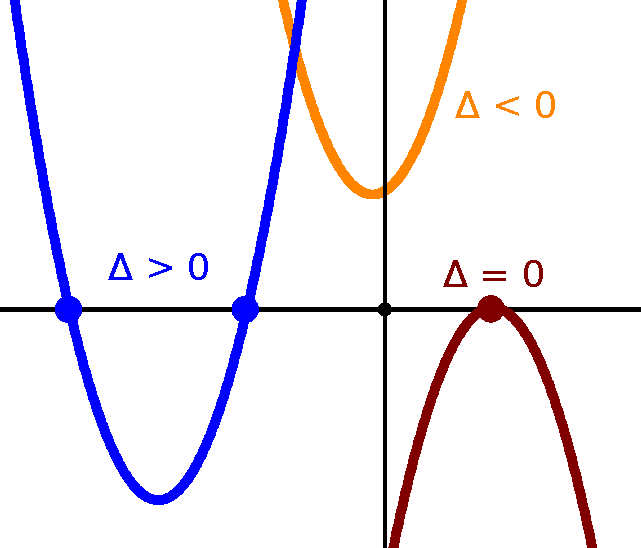
\includegraphics[width=0.5\textwidth]{Quadratic_eq_discriminant.pdf}
\end{center}
\caption{Examples of quadratic functions with zero, one and two real roots.}
\label{DisFig}
\end{figure}


\end{document}
